\documentclass[12pt]{article}
\usepackage{multicol}
\usepackage{subcaption}
\usepackage{natbib}
\bibliographystyle{plainnat}
\usepackage{amsmath}
\usepackage{graphicx}
\usepackage{setspace}
\doublespacing


\title{CIC Placement and Reporting Effects}
\author{Andrew Zilles}
\date{1 May 2024}

\begin{document}

\maketitle

\begin{abstract}
This study explores how audits conducted by the Internal Revenue Service (IRS) influence firms' reporting decisions. Utilizing a framework established by Ayers, Seidman, and Towery\citep{Ayers2019}, I seek to add context to the application of existing accounting theories by comparing firms subject to certain IRS audits with those that are not. My research addresses the core question of how IRS audits impact the reporting behavior of firms and explores the trade offs between increased tax compliance audits and publicly available information for investors.
\end{abstract}

\section{Introduction}
There exists in the current accounting literature a belief that firms wish to disclose more information to the public, but are afraid to do so for fear of audit by the Internal Revenue Service (IRS).

\begin{quote}
"Furthermore, we conjecture that some managers may simply be \textbf{unable to credibly communicate information} about the firm's tax planning without \textbf{divulging too much information to the tax authorities}." \citep{Balakrishnan2019} (emphasis added)
\end{quote}

\begin{quote}
"Further, managers cannot costlessly disclose the accrual because \textbf{the tax authority could use that information} to pursue additional claims" \citep{Dhaliwal2004} (emphasis added)
\end{quote} 

Intuitively, it makes sense that firms would choose to disclose less if they perceived this as leading to a higher probability of audit. However, many of the largest firms are under certain audit due to the Coordinated Industry Case (CIC) program of the IRS. This means that an IRS agent is frequently on site, sometimes with their own office provided by the firm, using the same break room as the firm's employees, and having regular discussion with tax departments and management about the implications of transactions. There is still a line of separation between the IRS agent and the firm. IRS agents must remain independent and are not permitted to consult firms about how they can and cannot operate - only on the tax implications of their decisions. But their availability calls into question the idea that firms aren't disclosing information because it might "tip off" the IRS.

\vspace{\baselineskip}

I seek to study the relationship between firm disclosures and certain audit by the IRS. My results do not conflict with the underlying theory that firms will strategically disclose if it could increase the possibility of audit. Instead, I examine the reporting and communication behaviors of firms that no longer have to calculate an audit probability because it is certain and compare it with firms who have audit uncertainty. I seek to answer if certain audit firms disclose and report differently than uncertain audit firms.

\section{Literature Review}
Taxpayer compliance models have already been established in the literature. These models express compliance as a function of tax rates, detection probability and punishment, and penalties and taxpayer risk-aversion. \citep{Allingham1972} These models have been extended multiple times to include various attributes of the audit relationship, notably: certain and verifiable information that allows the IRS to better focus audits\citep{Sansing1993}, the impact of a prior audit decision on current audit decision\citep{Rhoades1999}, and the differences between book and tax income\citep{Mills2000}.

\vspace{\baselineskip}

However, the effect of certain audit on these models is unclear since they only look at increasing the probability of audit. If audit probability is already set to 100\%, there is no way for it to increase. The implications of this are further explained by Ayers, Seidman, and Towery:
\begin{quote}
"Specifically, because the IRS will audit the firm regardless of the level of tax planning, certain audit firms no longer have incentive to reduce their tax planning to avoid IRS audit selection. This suggests audit certainty could result in increased tax uncertainty" \citep{Ayers2019}
\end{quote}

It is difficult to examine if a firm's disclosure lead to an IRS audit or not. Tax compliance audits are private information and are not disclosed by the IRS. However, the structure, resources, and policies of the IRS are publicly available. The IRS has a Large Businesses \& International (LB\&I) division with substantial resources and has been operating a Coordinated Industry Cases (CIC) program in various forms since the 1960s. The CIC progam ensures that the largests and most complex companies are audited every year. This is seen as a mutually beneficial arrangement: firms can remove the risk of uncertainty that their tax reporting will produce a significant and unexpected tax liability and the IRS can more effectively plan and deploy their limited resources to increase compliance and reporting quality.

\vspace{\baselineskip}

The participants in the CIC program are not publicly disclosed by the IRS, but the criteria examined when making CIC assignments has been disclosed in IRM Exhibit 4.46.2-2. These include various items such as amount of sales, total assets, number of foreign segments, business complexity, and amount of foreign taxes paid. Ayers et al. were able to examine IRS data and review the companies participating in the CIC program. They shared that this program captured a significant portion of the market:
\begin{quote} "We estimate that firms assigned to the CIC program account for between 65 and 70 percent of the U.S. market capitalization in 2011." \citep{Ayers2019}
\end{quote}
Following that review, they created a template that could be used by researchers using publicly available data reported by the firm.\citep{Ayers2019} I utilize this template to determine CIC assignment and then examine if firms facing certain audit change their reporting behaviors.
\vspace{\baselineskip}

To summarize, firms are faced with choices of what to report, how much to report, and how it should be reported. They strategically report or do not report information based on their risk preferences and probability of detection by the IRS. However, when risk of audit becomes certain, firms may change their disclosure strategy. I seek to examine this relationship more by using the CIC program established by the IRS. This program was designed so that large and complex businesses are subject to certain audit. I examine the reporting behaviors of firms in this program using the template established by Ayers et al. compared to firms outside this program to find if certain audit impacts a firm's reporting strategy.

\section{Data}
In order to test my research question, I utilize Compustat Segments and Fundamental Annual through WRDS. Compustat is a collection of annual financial data released by publicly traded companies. It is helpful for collecting information from all firms into a single location. However, since there are multiple data tables within Compustat, some merging and slicing of data is necessary to get all necessary varaibles into a single observation.
\vspace{\baselineskip}

The first challenge was within the Compustat Segments dataset. This table stored all the different segment types in the same variable. I had to extract the observations for the segment types I wanted (business segments and geographic segments) and discard the segments I didn't need. Once those were extracted, I then needed to get a count for how many of each segment were included. Taking it a step further, I then needed to identify which segments were foreign and which were domestic. This was fairly easy since most segments were labeled "United States." However, I did have to make the assumption that if a segment was labeled "North America" it was primarily United States even though it could include amounts for Canada, Mexico, or other Latin American countries. I only allowed this assumption when there wasn't a "United States" value and I knew from the data in Compustat that each firm has a segment in the United States. I then summed all the non-United States sales percents to come up with a total percent of foreign sales figure.
\vspace{\baselineskip}

Once the date for number of segments was created, I had to merge that with annual financial data from Fundamental Annual. I merged these on a unique firm identifier provided by Compustat and made sure that they were correctly merging together by firm and year. Since firms could change their reporting segments from year to year, it was important that I was merging Segments data with Fundamental Annual data on a firm-year basis. I then needed to calculate the amount of foreign sales by multiplying the total sales amount from Fundamental Annual with the percent of foreign sales calculated above.
\vspace{\baselineskip}

Now that all the variables are in a single dataset, I followed the method laid out by Ayers et al. to determine if a firm was in the CIC program or not.\citep{Ayers2019} Their method is based on IRM Exhibit 4.46.2-2 and is based on a point system. See Appendix~\ref{app:IRM} at the end for a breakdown of how points are assigned. After coding in these point vales based on the related Compustat variable with many nested ifelse statements and a sum of all attribute points, I created a dummy variable equal to 1 if the firm had more than 12 points. This represents if the firm is in the CIC program and is facing certain audit. Similar to \citep{Ayers2019} I also limit my sample to fiscal years 2007-2011 and firms with more than \$250 million in total assets. These limitations were added because of a regulation change in 2007 that could impact the results and to filter out small companies with complex operations that would be ignored by the IRS. (Although the IRM and official guidance by the IRS do not specifically state that a firm must meet a \$250 million threshold to be considered for the program, unofficially the IRS and an IRS director have commented that firms below this amount would not be considered large.
\vspace{\baselineskip}

Here I acknowledge my use of AI with Claude and ChatGPT helping me write some of the code to obtain the data and clean it up. I worked to understand the output provided by these tools and ensure that it was calculating my variables correctly. Some of the simpler lines of code were auto completed within R using Github Copilot (such as assigning point values to the different categories.)

\section{Methods}
Prior literature has identified size and complexity as determinants of CIC assignment.\citep {Mills1998} \citep{Hanlon2007} These attributes are simple, and we present this in our first equation.
\vspace{\baselineskip}

\begin{center}
\(CICFirm = \alpha  + \beta Size + \gamma Complexity + \epsilon\)

\begin{equation}
\label{eq:CICSimple}
\end{equation}
\end{center}
\vspace{\baselineskip}

Expanding on this model, we examine the attributes from the Internal Revenue Manual (IRM) Exhibit 4.46.2-2 with suggestions from Ayers et al.\citep{Ayers2019} The seven characteristics defined by the IRM are:
\begin{enumerate}
   \item Total Assets
   \item Gross Receipts
   \item Operating Entities
   \item Multiple Industry Status
   \item Total Foreign Assets
   \item Total Related Transactions
   \item Foreign Tax
\end{enumerate}

Unfortunately, there is no publicly available proxy for item 6, Total Related Transactions, so it is dropped from equation 2. Total Foreign Assets has also been replaced with a calculation of Total Foreign Sales, due to its availability and the similarity between assets and sales. Further, I rename the variables in equation 2 to better align with their counterparts in Compustat, the database of publicly available financial information.
\begin{enumerate}
   \item Assets, Total
   \item Sales
   \item Number of Geographic Segments (GEOSEG)
   \item Number of Business Segments (BUSSEG)
   \item Sales * Foreign Sales Percentage
   \item Dropped
   \item Tax Expense, Foreign
\end{enumerate}

Each of these can be categorized into Size and Complexity variables. We add these designations to our first equation above.
\vspace{\baselineskip}
\begin{center}
\(CICFirm = \alpha  + \beta_1 \text{AssetPoints}  + \beta_2 \text{GrossReceiptsPoints} + \gamma_1 \text{GeoSegPoints} + \gamma_2 \text{BusSegPoints} + \gamma_3 \text{ForeignSalesPoints} + \gamma_4 \text{ForeignTaxPoints} + \epsilon\)
\begin{equation}
\label{eq:CICComp}
\end{equation}
\end{center}
\vspace{\baselineskip}

This is where I acknowledge a break from what I've said prior. I intend to write this as my first year summer paper as part of my PhD program. I want to explore the relationship between how firms communicate and if they face audit certainty. That analysis is going to take a lot more work and setup than what I currently have time to give for this project. So instead of pulling in data from firms' 10-Ks, 10-Qs, earnings calls, and other disclosures and feed it through textual analysis tools provided by the University of Notre Dame, I'm instead going to simplify my approach and just look at a regression on the above variables. That means this paper isn't really about how firms communicate and is instead about what factors contribute to the firm being selected for the CIC program. I want to confirm that these factors are all important and that they are not dominated by one variable.
\vspace{\baselineskip}

In order to do this, I regress equation 2 above using GLM function and with a logit link. This will allow us to determine which factors are important.


\section{Findings}
I will start by sharing the summary statistics and then discuss the regression results. These are presented in Table \ref{tab:Summary} and Table \ref{tab:Regression}, respectively. The regression results from Table \ref{tab:Regression} show that all variables are significant at the 1\% level with positive coefficients. This result is a little unsurprising given that these variables are all used when determining the value of CIC placement.
\vspace{\baselineskip}

To show the distribution of firms in the CIC program versus those without, I create Figure \ref{fig:Dist}. This figure shows the number of firm year observations for firms in the CIC program (CIC = 1) compared to firm year observations out of the CIC program (CIC = 0).
\vspace{\baselineskip}

To further explore these results I regress equation 2 again, but this time include variables for other common tax complexity indicators. These include how much Leverage a company has (debt vs equity financing), the Capital Investment intensity (for depreciation and R\&D tax credits), Excessive Stock Compensation (for reduced labor expense), and Net Operating Losses (for Loss carryforwards/carrybacks.) The results are shown in Table \ref{tab:Regression2}. The CIC determinant coefficients are all positively related still witth significance at the 1\% level. Leverage and Capital Intensity are also statistically significant at the 10\% level, but this could simply be due to their relationship with Total Assets. Unsurprisingly stock compensation and operating losses are not significant. The results are again a little underwhelming, but confirm that all components are important when determining CIC placement and are not dominated by a few high profile metrics.


\section{Conclusion}
Following the simple regressions, we can see that placement in the CIC program is driven by all of the factors described by Ayers et al. \citep{Ayers2019} We are not yet able to comment on how firms respond to audit certainty and if they adjust their reporting behavior or not. I plan to continue this research in the future by pulling in textual analysis and firm's 10-K, 10-Q, conference call transcripts, and various other means of communication to determine if firms who face audit certainty communicate differently. 

\section{Bibliography}
\nocite{*}
\bibliography{FinalProjectBibliography_Zilles}

\vspace{\baselineskip}
\vspace{\baselineskip}
\vspace{\baselineskip}
\vspace{\baselineskip}


%%%%%%%%%% Appendix 1
\appendix
\section{IRM exhibit 4.46.2-2}
\label{app:IRM}
\centering

\vspace{\baselineskip}
1. Total Assets (COMPUSTAT AT, IRS 4.46.2-2 point system)
\begin{itemize}
   \item 1 point for up to \$500 million in assets;
   \item 2 points for assets in the \$500 million to \$1 billion range;
   \item 3 points for assets in the \$1 billion to \$2 billion range;
   \item 4 points for assets in the \$2 billion to \$5 billion range;
   \item 5 points for assets in the \$5 billion to \$8 billion range;
   \item Add 1 point for each additional \$3 billion in assets, or fraction thereof, not to exceed 12 points.
\end{itemize}
\vspace{\baselineskip}

2. Gross Receipts (COMPUSTAT SALE, IRS 4.46.2-2 point system)
\begin{itemize}
   \item 1 point for up to \$1 billion in gross receipts;
   \item 2 points for gross receipts in the \$1 billion to \$2 billion range;
   \item 3 points for gross receipts in the \$2 billion to \$3 billion range;
   \item 4 points for gross receipts in the \$3 billion to \$5 billion range;
   \item 5 points for gross receipts in the \$5 billion to \$10 billion range;
   \item Add one point for each additional \$3 billion in gross receipts, or fraction thereof, not to exceed 10 points.
\end{itemize}
\vspace{\baselineskip}

3. Operating Entities (geographic segments from COMPUSTAT Segments data set, IRS 4.46.2-2 point system)
\begin{itemize}
   \item 1 point for 1 entity;
   \item 3 points for 2--5 entities;
   \item 5 points for 6--9 entities;
   \item 7 points for 10--13 entities;
   \item 9 points for more than 13 entities.
\end{itemize}
\vspace{\baselineskip}

4. Multiple Industry Status (business segments from COMPUSTAT Segments data set, point system based on point system for Operating Entities because IRM Exhibit is not detailed for this item)
\begin{itemize}
   \item 1 point for 1 industry;
   \item 3 points for 2--5 industries;
   \item 5 points for 6--9 industries;
   \item 7 points for 10--13 industries;
   \item 9 points for more than 13 industries.
\end{itemize}
\vspace{\baselineskip}

5. Total Foreign Assets (we substitute foreign sales for foreign assets; foreign sales percentage from COMPUSTAT Segments data set times COMPUSTAT SALE; modified point system)
\begin{itemize}
   \item 1 point up to \$500 million in foreign sales;
   \item 2 points for foreign sales in the \$500 million to \$1 billion range;
   \item 3 points for foreign sales in the \$1 billion to \$1.5 billion range;
   \item 4 points for foreign sales in the \$1.5 billion to \$2.5 billion range;
   \item 5 points for foreign sales in the \$2.5 billion to \$5 billion range;
   \item Add 1 point for each additional \$1.5 billion in foreign sales, or fraction thereof, not to exceed 8 points.
\end{itemize}
\vspace{\baselineskip}

6. Total Related Transactions
\textit{Unable to create a publicly available proxy} \\
\vspace{\baselineskip}

7. Foreign Tax (COMPUSTAT TXFO, IRS 4.46.2-2 point system)
\begin{itemize}
   \item 1 point up to \$7 million in foreign tax;
   \item 2 points for foreign tax in the \$7 million to \$100 million range;
   \item 3 points for foreign tax in the \$100 million to \$200 million range;
   \item Add 1 point for each additional \$100 million in foreign tax, or fraction thereof, not to exceed 7 points.
\end{itemize}
\vspace{\baselineskip}
\vspace{\baselineskip}


%%%%%%%%%% Figure 1
\begin{figure}[htbp]
    \centering
    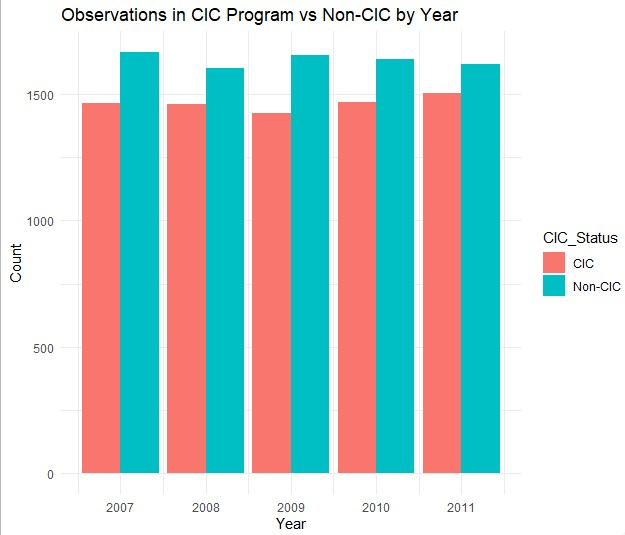
\includegraphics[width=1\linewidth]{Graph.jpg}
    \caption{Distribution of firm-year observations in the CIC program versus non-CIC firms.}
    \label{fig:Dist}
\end{figure}



%%%%%%%%%% Table 1
% latex table generated in R 4.3.2 by xtable 1.8-4 package
% Mon May  6 19:15:35 2024
\begin{table*}[p]
\caption{Summary Statistics}
\label{tab:Summary}
\centering
\begin{tabular}[t]{lrrrrrr}
  \hline
Variable & Count & Median & Mean & SD & Min & Max \\ 
  \hline
  at & 15501 & 1653.151 & 15829.659 & 115699.588 & 250.035 & 3221972.000 \\ 
  sale & 15501 & 865.248 & 5384.854 & 19517.307 & -15009.328 & 470171.000 \\ 
  BUSSEG & 15501 & 1.000 & 2.340 & 1.766 & 1.000 & 11.000 \\ 
  GEOSEG & 15501 & 2.000 & 2.709 & 2.674 & 1.000 & 28.000 \\ 
  ForeignSales & 15501 & 40.050 & 2340.212 & 12598.800 & -16346.967 & 378225.000 \\ 
  ForeignTax & 15501 & 0.000 & 41.932 & 531.900 & -2751.000 & 32666.000 \\ 
  CICFirm & 15501 & 0.000 & 0.472 & 0.499 & 0.000 & 1.000 \\ 
   \hline
\end{tabular}
\end{table*}




%%%%%%%%%% Table 2
% latex table generated in R 4.3.2 by xtable 1.8-4 package
% Mon May  6 20:34:52 2024
\begin{table}[ht]
\centering
\caption{Regression of CIC program characteristics}
\label{tab:Regression}
\begin{tabular}{crrrr}
  \hline
Coefficient & Estimate & Std. Error & z value & Pr(>|z|) \\ 
  \hline
  (Intercept) & -10.694 & 0.242 & -44.149 & 0.000 \\ 
  Total Assets & 0.001 & 0.000 & 32.210 & 0.000 \\ 
  Sales & 0.002 & 0.000 & 34.497 & 0.000 \\ 
  Geographic Segments & 0.913 & 0.030 & 30.834 & 0.000 \\ 
  Business Segments & 1.172 & 0.035 & 33.695 & 0.000 \\ 
  Foreign Sales & 0.004 & 0.000 & 19.380 & 0.000 \\ 
  Foreign Tax & 0.025 & 0.002 & 12.574 & 0.000 \\ 
   \hline
\end{tabular}
\end{table}




%%%%%%%%%% Table 3
% latex table generated in R 4.3.2 by xtable 1.8-4 package
% Mon May  6 21:10:05 2024
\begin{table}[ht]
\centering
\caption{Regression of CIC program characteristics with other common tax indicators}
\label{tab:Regression2}
\begin{tabular}{crrrr}
  \hline
Coefficient & Estimate & Std. Error & z value & Pr(>|z|) \\ 
  \hline
(Intercept) & -10.846 & 0.264 & -41.153 & 0.000 \\ 
  Total Assets & 0.001 & 0.000 & 30.533 & 0.000 \\ 
  Sales & 0.002 & 0.000 & 32.756 & 0.000 \\ 
  Geographic Segments & 0.926 & 0.031 & 30.012 & 0.000 \\ 
  Business Segments & 1.161 & 0.035 & 32.758 & 0.000 \\ 
  Foreign Sales & 0.004 & 0.000 & 18.912 & 0.000 \\ 
  Foreign Tax & 0.025 & 0.002 & 12.732 & 0.000 \\  
  Leverage & 0.333 & 0.177 & 1.879 & 0.060 \\ 
  Capital Intensity & 0.326 & 0.175 & 1.864 & 0.062 \\ 
  Excessive Stock Compensation & 0.036 & 0.091 & 0.390 & 0.697 \\ 
  Net Operating Loss & -0.086 & 0.091 & -0.954 & 0.340 \\ 
   \hline
\end{tabular}
\end{table}



\end{document}
